\documentclass[12pt, a4paper]{article}
\usepackage{amsmath, amsfonts}
\usepackage[utf8]{inputenc}
\usepackage[russian]{babel}
\usepackage{graphicx}
\usepackage{wrapfig}
\usepackage{geometry}
\usepackage[indentfirst,compact,topmarks,calcwidth,pagestyles]{titlesec}
\usepackage{verbatim}
\usepackage{titletoc}
\usepackage{cmap}
\geometry{verbose, a4paper, top=2cm, bottom=2cm, left=2cm, right=2cm}
\begin{document}
\section{Постановка задачи}
\begin{wrapfigure}{r}{0.4\textwidth}
  \centering
  \label{fig:1}
  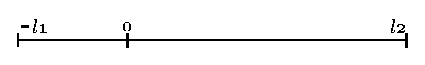
\includegraphics[width=0.38\textwidth]{fig1.eps}
  \\
  \caption{Двухслойный стержень}
\end{wrapfigure}
В данной работе решается задача диффузии-конвекции для одномерной конечной двухслойной области, которая схематически показана на Рис.~\ref{fig:1}. Для удобства граница раздела слоев помещена в начало координат.

Математическая постановка задачи состоит в следующем: требуется решить уравнение в частных производных
\begin{equation}
 u_t = wu_x + a^2 u_{xx} 
 \label{eq:12}
\end{equation}
с однородным начальным условием
\begin{equation}
 u(x,0) = 0 
\end{equation}
а также внешними и общими граничными условиями 
\begin{equation}
  \left\{
  \begin{aligned}
    & u(-l_1,t) = 1 - \cos \omega t, \\
    & u_x(l_2,t) = 0, \\
    & u(-0, t) = u(+0, t), \\
    & a_1^2 u_{x}(-0, t) = a_2^2 u_{x}(+0, t), \\
  \end{aligned}
  \right.
\end{equation}
где $a(x)$, $w(x)$ --- кусочно-постоянные коэффициенты диффузии и скорости осаждения соответственно:
\begin{equation}
  a=a(x)=\left\{ 
    \begin{aligned}
      & a_1\ \text{при}\ x \in [-l_1;0), \\
      & a_2\ \text{при}\ x \in [0;l_2], \\
    \end{aligned}
\right.
\end{equation}
\begin{equation}
  w=w(x)=\left\{ 
    \begin{aligned}
      & w_1\ \text{при}\ x \in [-l_1;0), \\
      & w_2\ \text{при}\ x \in [0;l_2]. \\
    \end{aligned}
\right.
\end{equation}
\section{Решение}
\subsection{Переход к однородным граничным условиям}
Для перехода к однородным граничным условиям производим замену
\begin{equation}
  u(x,t) = N(x,t) + (1 - \cos \omega t).
\end{equation}
В результате приходим к новому уравнению, начальному и граничным условиям
\begin{equation}
  N_t(x,t) = w N_x(x,t) + a^2 N_{xx}(x,t) - \omega\sin\omega t,
  \label{eq:14}
\end{equation}
\begin{equation}
  N(x,0) = 0,
\end{equation}
\begin{equation}
  \left\{
  \begin{aligned}
    & N(-l_1,t) = 0, \\
    & N_x(l_2,t) = 0, \\
    & N(-0, t) = N(+0, t), \\
    & a_1^2 N_{x}(-0, t) = a_2^2 N_{x}(+0, t). \\
  \end{aligned}
  \right.
  \label{eq:15}
\end{equation}
\subsection{Разделение переменных}
Пусть $ N(x,t)=\theta(t)\varphi(x) $, тогда
\begin{equation}
  \frac{\theta'}{\theta}=\frac{a^2\varphi''+w\varphi'}{\varphi}=k.
  \label{eq:1}
\end{equation}
Константа $ k $ не может быть положительной, в противном случае $\lim_{t \rightarrow \infty}\theta(t) \ne 0$, что противоречит физическому смыслу задачи. Ввиду этого, можно принять
\begin{equation}
  k=-\beta^2.
  \label{eq:2}
\end{equation}
\subsection{Задача Штурма--Лиувилля}
\subsubsection{Исключение конвективного слагаемого}
Из (\ref{eq:1}) и (\ref{eq:2}) следует задача Штурма--Лиувилля для $\varphi(x)$:
\begin{equation}
  a^2 \varphi''(x) + w \varphi'(x) + \beta^2\varphi(x)=0 \\
\end{equation}
с внешними граничными условиями и условиями сопряжения:
\begin{equation}
  \left\{
  \begin{aligned}
    & \varphi_1(-l_1) = 0, \\
    & \varphi_2'(l_2) = 0, \\
и   & \varphi_1(0) = \varphi_2(0), \\
    & a_1^2 \varphi_1'(0) = a_2^2 \varphi_2'(0). \\
  \end{aligned}
  \right.
  \label{eq:16}
\end{equation}
Здесь
\begin{equation}
  \varphi(x)=\left\{ 
    \begin{aligned}
      & \varphi_1(x)\ \text{при}\ x \in [-l_1;0), \\
      & \varphi_2(x)\ \text{при}\ x \in [0;l_2]. \\
    \end{aligned}
\right.
\end{equation}

Для того чтобы исключить из уравнения слагаемое $w\varphi'(x)$, производим замену 
\begin{equation}
  \varphi(x) = \psi(x) e^{- \mu x},\ \text{где}\ \mu=\mu(x) = \left\{
    \begin{aligned}
      & \mu_1 = \frac{w_1}{2a_1^2}\ \text{при}\ x \in [-l_1;0), \\
      & \mu_2 = \frac{w_2}{2a_2^2}\ \text{при}\ x \in [0;l_2]. \\
    \end{aligned}
    \right.
\end{equation}
В итоге получаем новое уравнение
\begin{equation}
  a^2\psi''(x) + (\beta^2 - \mu^2a^2) \psi(x) = 0
  \label{eq:3}
\end{equation}
и новые граничные условия
\begin{equation}
  \left\{
  \begin{aligned}
    & \psi_1(-l_1) = 0, \\
    & \psi_2'(l_2) - \mu\psi_2(l_2) = 0, \\
    & \psi_1(0) = \psi_2(0), \\
    & a_1^2(\psi_1'(0) - \mu\psi_1(0)) =  a_2^2(\psi_2'(0) - \mu\psi_2(0)). \\
  \end{aligned}
  \right.
  \label{}
\end{equation}

Пусть для определенности $\mu_1 \le \mu_2$. Тогда для нахождения собственных чисел $\beta$ необходимо рассмотреть три отрезка. Собственным числам из разных отрезков будет соответствовать разный вид собственных функций
\begin{enumerate}
  \item $ 0 \le \beta \le \mu_1a_1, $
  \item $ \mu_1a_1 < \beta \le \mu_2a_2, $
  \item $ \mu_2a_2 < \beta < \infty. $
\end{enumerate}
\subsubsection{Нахождение собственных чисел и собственных функций}
\framebox{i} $ 0 \le \beta \le \mu_1a_1$. Собственные функции $\psi$ будут иметь вид:
\begin{equation}
  \begin{aligned}
    \psi_1(x) = A_1 \ch q_1x + B_1 \sh q_1x, \\
    \psi_2(x) = A_2 \ch q_2x + B_2 \sh q_2x.
  \end{aligned}
  \label{eq:5}
\end{equation}
Где 
\begin{equation}
  \begin{aligned}
    q_1 = q_1(\beta) = \sqrt{- \frac{\beta^2}{a_1^2} + \mu_1}, \\
    q_2 = q_2(\beta) = \sqrt{- \frac{\beta^2}{a_2^2} + \mu_2}.
  \end{aligned}
\end{equation}
Константы $A_1$, $A_2$, $B_1$, $B_2$ определяем из граничных условий. Используя граничные условия, получим:
\begin{equation}
  \left\{  
  \begin{aligned}
    & A_1 \ch q_1l_1 - B_1 \sh q_1l_1 = 0, \\
    & A_2 (q_2\sh q_2l_2 - \mu_2\ch q_2l_2) + B_2 (q_2\ch q_2l_2 - \mu_2\sh q_2l_2) = 0, \\
    & A_1 = A_2, \\
    & A_1 (-\mu_1a_1^2) + B_1 (q_1a_1^2) = A_2 (-\mu_2a_2^2) + B_2 (q_2a_2^2).
  \end{aligned}
  \right.
  \label{eq:4}
\end{equation}
Чтобы найти ненулевые коэффициенты $A_i$, $B_i$, необходимо, чтобы определитель системы уравнений (\ref{eq:4}) относительно $A_i$, $B_i$ был равен нулю. В результате получим уравнение для $\beta$:
\begin{equation}
  \det \left(  
  \begin{smallmatrix}
    \ch(q_1(\beta) l_1) & 0 & -\sh(q_1(\beta) l_1) & 0 \\
    0 & q_2(\beta) \sh(q_2(\beta) l_2)-\ch(q_2(\beta) l_2) \mu_2 & 0 & q_2(\beta) \ch(q_2(\beta) l_2)-\sh(q_2(\beta) l_2) \mu_2 \\
    1 & -1 & 0 & 0 \\
    -a_1^2 \mu_1 & a_2^2 \mu_2 & a_1^2 q_1(\beta) & -a_2^2 q_2(\beta) \\
  \end{smallmatrix}
  \right) = 0,
\end{equation}
или в развернутом виде
\begin{equation}
  \begin{aligned}
  & -\sh(q_1(\beta) l_1) ((a_2^2 \mu_2-a_1^2 \mu_1) (q_2(\beta) \ch(q_2(\beta) l_2)-\sh(q_2(\beta) l_2) \mu_2)+a_2^2 q_2(\beta)- \\
  & -(q_2(\beta) \sh(q_2(\beta) l_2)-\ch(q_2(\beta) l_2) \mu_2))-a_1^2 q_1(\beta) \ch(q_1(\beta) l_1) \times \\
  & \times (q_2(\beta) \ch(q_2(\beta) l_2)-\sh(q_2(\beta) l_2) \mu_2) = 0.
  \end{aligned}
\end{equation}
После определения собственных чисел, из системы (\ref{eq:4}) находим коэффициенты $A_i$, $B_i$
\begin{equation}
  \begin{aligned}
    & A_1 = A_2 = \sh q_1l_1, \\
    & B_1 = \ch q_1l_1, \\
    & B_2 = \frac{\sh (q_1l_1) (-\mu_1 a_1^2 + \mu_2 a_2^2) + \ch (q_1l_1) q_1 a_1^2}{q_2a_2^2}.
  \end{aligned}
\end{equation}
Таким образом, найден набор собственных функций (\ref{eq:5}), соответствующий отрезку $ 0 \le \beta \le \mu_1a_1 $.

\framebox{ii} $ \mu_1a_1 < \beta \le \mu_2a_2 $. Аналогичным образом определяем собственные числа и функции для случая $ \mu_1a_1 < \beta \le \mu_2a_2 $:
\begin{equation}
  \begin{aligned}
    & \psi_1(x) = A_1 \cos q_1x + B_1 \sin q_1x, \\
    & \psi_2(x) = A_2 \ch q_2x + B_2 \sh q_2x, \\
    & q_1 = q_1(\beta) = \sqrt{\frac{\beta^2}{a_1^2} - \mu_1}, \\
    & q_2 = q_2(\beta) = \sqrt{- \frac{\beta^2}{a_2^2} + \mu_2}.
  \end{aligned}
  \label{eq:6}
\end{equation}
\begin{equation}
  \det \left(  
  \begin{smallmatrix}
    \cos(q_1(\beta) l_1) & 0 & -\sin(q_1(\beta) l_1) & 0 \\
    0 & q_2(\beta) \sh(q_2(\beta) l_2)-\ch(q_2(\beta) l_2) \mu_2 & 0 & q_2(\beta) \ch(q_2(\beta) l_2)-\sh(q_2(\beta) l_2) \mu_2 \\
    1 & -1 & 0 & 0 \\
    -a_1^2 \mu_1 & a_2^2 \mu_2 & a_1^2 q_1(\beta) & -a_2^2 q_2(\beta) \\
  \end{smallmatrix}
  \right) = 0.
\end{equation}
\begin{equation}
  \begin{aligned}
  & -\sin(q_1(\beta) l_1) ((a_2^2 \mu_2-a_1^2 \mu_1) (q_2(\beta) \ch(q_2(\beta) l_2)-\sh(q_2(\beta) l_2) \mu_2)+a_2^2 q_2(\beta)- \\
  & -(q_2(\beta) \sh(q_2(\beta) l_2)-\ch(q_2(\beta) l_2) \mu_2))-a_1^2 q_1(\beta) \cos(q_1(\beta) l_1) \times \\
  & \times (q_2(\beta) \ch(q_2(\beta) l_2)-\sh(q_2(\beta) l_2) \mu_2) = 0.
  \end{aligned}
\end{equation}
\begin{equation}
  \begin{aligned}
    & A_1 = A_2 = \sin q_1l_1, \\
    & B_1 = \cos q_1l_1, \\
    & B_2 = \frac{\sin (q_1l_1) (-\mu_1 a_1^2 + \mu_2 a_2^2) + \cos (q_1l_1) q_1 a_1^2}{q_2a_2^2}.
  \end{aligned}
\end{equation}

\framebox{iii} $\mu_1a_1 < \beta < \infty$. Собственные функции, уравнения для собственных значений, постоянные $A_i$, $B_i$ имеют вид:
\begin{equation}
  \begin{aligned}
    & \psi_1(x) = A_1 \cos q_1x + B_1 \sin q_1x, \\
    & \psi_2(x) = A_2 \cos q_2x + B_2 \sin q_2x, \\
    & q_1 = q_1(\beta) = \sqrt{\frac{\beta^2}{a_1^2} - \mu_1}, \\
    & q_2 = q_2(\beta) = \sqrt{\frac{\beta^2}{a_2^2} - \mu_2}.
  \end{aligned}
  \label{eq:7}
\end{equation}
\begin{equation}
  \det \left(  
  \begin{smallmatrix}
    \cos(q_1(\beta) l_1) & 0 & -\sin(q_1(\beta) l_1) & 0 \\
    0 & - q_2(\beta) \sin(q_2(\beta) l_2)-\cos(q_2(\beta) l_2) \mu_2 & 0 & q_2(\beta) \cos(q_2(\beta) l_2)-\sin(q_2(\beta) l_2) \mu_2 \\
    1 & -1 & 0 & 0 \\
    -a_1^2 \mu_1 & a_2^2 \mu_2 & a_1^2 q_1(\beta) & -a_2^2 q_2(\beta) \\
  \end{smallmatrix}
  \right) = 0.
\end{equation}
\begin{equation}
  \begin{aligned}
    & -\sin(q_1(\beta) l_1) ((a_2^2 \mu_2-a_1^2 \mu_1) (q_2(\beta) \cos(q_2(\beta) l_2)-\sin(q_2(\beta) l_2) \mu_2)+ \\
    & + a_2^2 q_2(\beta) (-\cos(q_2(\beta) l_2) \mu_2-q_2(\beta) \sin(q_2(\beta) l_2)))- \\
    & -a_1^2 q_1(\beta) \cos(q_1(\beta) l_1) (q_2(\beta) \cos(q_2(\beta) l_2)-\sin(q_2(\beta) l_2) \mu_2) = 0.
  \end{aligned}
\end{equation}
\begin{equation}
  \begin{aligned}
    & A_1 = A_2 = \sin q_1l_1, \\
    & B_1 = \cos q_1l_1, \\
    & B_2 = \frac{\sin (q_1l_1) (-\mu_1 a_1^2 + \mu_2 a_2^2) + \cos (q_1l_1) q_1 a_1^2}{q_2a_2^2}.
  \end{aligned}
\end{equation}
\subsection{Ортогональность собственных функций}
Собственные функции (\ref{eq:5}), (\ref{eq:6}), (\ref{eq:7}), как решения задачи Штурма--Лиувилля ортогональны с весом $\rho_\psi=\rho_\psi(x)$. Покажем, что $\rho_\psi=1$, проделав следующие преобразования:
Пусть $n \ne m$
\begin{equation}
  \left\{  
    \begin{aligned}
      & a^2 \psi_n'' + (\beta_n^2 - \mu^2 a^2) \psi_n = 0, \\
      & a^2 \psi_m'' + (\beta_m^2 - \mu^2 a^2) \psi_m = 0. \\
    \end{aligned}
  \right.
  \label{eq:8}
\end{equation}
Первое уравнение (\ref{eq:8}) умножим на $\psi_m$ и проинтегрируем на отрезке $[-l_1; l_2]$. Аналогично, второе уравнение умножим на $\psi_n$ и проинтегрируем на том же отрезке
\begin{equation}
  \left\{  
    \begin{aligned}
      & \int \limits^{l_2}_{-l_1} a^2 \psi_n'' \psi_m dx = - \beta_n^2 \int \limits^{l_2}_{-l_1} \psi_n \psi_m dx + \int \limits^{l_2}_{-l_1} a^2 \mu^2 \psi_n \psi_m dx, \\
      & \int \limits^{l_2}_{-l_1} a^2 \psi_m'' \psi_n dx = - \beta_m^2 \int \limits^{l_2}_{-l_1} \psi_n \psi_m dx + \int \limits^{l_2}_{-l_1} a^2 \mu^2 \psi_n \psi_m dx. 
    \end{aligned}
  \right.
  \label{eq:9}
\end{equation}
Вычитая из первого уравнения (\ref{eq:9}) второе, получим 
\begin{equation}
  (\beta_m^2 - \beta_n^2) \int \limits^{l_2}_{-l_1} \psi_n \psi_m dx =  \int \limits^{l_2}_{-l_1} a^2 \psi_n'' \psi_m dx -  \int \limits^{l_2}_{-l_1} a^2 \psi_m'' \psi_n dx = I_1 - I_2.
  \label{eq:11}
\end{equation}
Дважды интегрируя $I_1$ по частям, имеем
\begin{equation}
  I_1 =  \int \limits^{l_2}_{-l_1} a^2 \psi_m d \psi_n' = \overbrace{a^2 \psi_m \psi_n' \Big|^{l_2}_{-l_1}}^P - \overbrace{a^2 \psi_n \psi_m' \Big|^{l_2}_{-l_1}}^Q + I_2 = P - Q + I_2.
\end{equation}
\begin{equation}
  I_1 - I_2 = P - Q.
  \label{eq:10}
\end{equation}
Учитывая граничные условия для $\psi_n$, $\psi_m$, найдем $P$:
\begin{equation}
  \begin{aligned}
    &P=a_2^2\overbrace{\psi_{2n}'(l_2)}^{\mu\psi_{2n}(l_2)}\psi_{2m}(l_2) - a_2^2 \psi_{2n}'(0) \psi_{2m}(0) + a_1^2 \psi_{1n}'(0) \psi_{1m}(0) - a_1^2 \psi_{1n}'(-l_1) \overbrace{\psi_{1m}(-l_1)}^0=\\
    & = \overbrace{a_2^2\mu\psi_{2n}(l_2)\psi_{2m}(l_2)}^{A} + \psi_{1m}(0)(a_1^2 \psi_{1n}'(0) - a_2^2\psi_{2n}'(0)) =\\
    & = A + \psi_{1m}(0)(\mu a_2^2 \psi_{2n}(0) - \mu a_1^2 \psi_{1n}(0)) = A + \mu \psi_{1m}(0)\psi_{1n}(0)(a_2^2 - a_1^2).
  \end{aligned}
\end{equation}
Из соображений симметрии $Q = P$, следовательно из (\ref{eq:10}) $I_1 = I_2$. Из (\ref{eq:11}) и предположения, что $n \ne m$ можно заключить, что
\begin{equation}
  \int \limits_{-l_1}^{l_2} \rho_\psi \psi_n(x) \psi_m(x) dx = 0
\end{equation}
Делая обратную замену для $\varphi = \psi e^{-\mu x}$, находим весовую функцию $\rho_\varphi$
\begin{equation}
  \int \limits_{-l_1}^{l_2} \varphi_n(x) \varphi_m(x) e^{2 \mu x} dx = \int \limits_{-l_1}^{l_2} \psi_n(x) \psi_m(x) dx = 0 \Rightarrow \rho_\varphi(x) = \rho(x) = e^{2 \mu x}.
\end{equation}
\subsection{Интегральное преобразование}
Решение вспомогательной задачи (\ref{eq:14})-(\ref{eq:15}) имеет вид 
\begin{equation}
  N(x,t)=\sum \limits_{n=1}^{\infty} \frac{\varphi_n(x) \theta_n(t)}{||\varphi_n||}.
\end{equation}
Где
\begin{equation}
  \theta_n(t) = \int \limits_{-l_1}^{l_2} \rho N(x,t) \varphi_n(x) dx.
  \label{eq:13}
\end{equation}
Для нахождения $\theta_n(t)$ необходимо провести интегральное преобразование обеих частей уравнения (\ref{eq:14}) с использованием формулы~(\ref{eq:13}):
\begin{equation}
  \begin{aligned}
    & \int \limits_{-l_1}^{l_2} \rho N_t \varphi_n dx = \overbrace{\int \limits_{-l_1}^{l_2} \rho w N_x \varphi_n dx}^{I_1} + \overbrace{\int \limits_{-l_1}^{l_2} \rho a^2 N_{xx} \varphi_n dx}^{I_2} +  \overbrace{\left( -\omega \sin \omega t \int \limits_{-l_1}^{l_2} \rho \varphi_n dx \right)}^{F(t)}  \Rightarrow \\
  & \Rightarrow \frac{\partial}{\partial t} \int \limits_{-l_1}^{l_2} \rho N \varphi_n dx = I_1 + I_2 + F(t) \Rightarrow \theta'(t) = I_1 + I_2 + F(t).
\end{aligned}
\end{equation}
При вычислении $I_1+I_2+F(t)$, принимаем во внимание, что $\rho'(x) = 2 \mu \rho(x)$.
\begin{equation}
  \begin{aligned}
    & I_2 = \int \limits_{-l_1}^{l_2} \rho a^2 \varphi_n d N_x = \overbrace{\rho a^2 \varphi_n N_x \Big|^{l_2}_{-l_1}}^P - 
    \int \limits_{-l_1}^{l_2} (2\mu\rho\varphi_n + \rho\varphi_n') a^2 N_x dx = P - \overbrace{\int \limits_{-l_1}^{l_2} 2 \mu \rho a^2 \varphi_n N_x dx}^{I_1} - \\
    & - \int \limits_{-l_1}^{l_2} \rho a^2\varphi_n'd N = P - I_1 - \overbrace{\rho a^2 \varphi_n' N \Big|^{l_2}_{-l_1}}^Q + 
    \int \limits_{-l_1}^{l_2} a^2 (2\mu\rho\varphi_n' + \rho\varphi_n'') N dx = P - Q - I_1 + \\
    & + \int \limits_{-l_1}^{l_2} \overbrace{(w\varphi_n' + a^2\varphi_n'')}^{-\beta_n^2\varphi_n} \rho N dx = P - Q - I_1 - \beta_n^2 \theta(t) \Rightarrow I_1 + I_2 + F(t) = P - Q - 
    \beta_n^2 \theta(t) + \\
    & + F(t) \Rightarrow \theta'(t) + \beta_n^2 \theta(t) = P - Q + F(t).
  \end{aligned}
  \label{eq:17}
\end{equation}
Используя граничные условия для $\varphi_n$ (\ref{eq:16}) и для $N(x,t)$ (\ref{eq:15}) определяем $P=Q=0$:
\begin{equation}
  \begin{aligned}
  & P = \rho(l_2) a_2^2 \varphi_{2n}(l_2) \overbrace{N_x(l_2)}^0 - \rho(-l_1) a_1^2 \overbrace{\varphi_{1n}(-l_1)}^0 N_x(-l_1) + \\
  & + \varphi_{1n}(0)\overbrace{(a_1^2 N_x(-0) - a_2^2 N_x(+0))}^0 = 0.
\end{aligned}
\end{equation}
\begin{equation}
  \begin{aligned}
    & Q = \rho(l_2) a_2^2 \overbrace{\varphi'_{2n}(l_2)}^0 N(l_2) - \rho(-l_1) a_1^2 \varphi'_{1n}(-l_1) \overbrace{N(-l_1)}^0 + \\
    & + N(0)\overbrace{(a_1^2 \varphi_{1n}'(0) - a_2^2 \varphi_{2n}'(0))}^0 = 0.
\end{aligned}
\end{equation}
Подставляем найденные значения в (\ref{eq:17})
\begin{equation}
\theta'(t) + \beta_n^2 \theta(t) = F(t).
\label{eq:18}
\end{equation}
\subsection{Нахождение временной составляющей решения}
Формула (\ref{eq:18}) является дифференциальным уравнением относительно функции $\theta_n(t)$. Начальное условие следует из соответствующего однородного начального условия для $N(x,t)$:
\begin{equation}
  \left\{  
  \begin{aligned}
    & \theta_n'(t) + \beta_n^2 \theta_n(t) = F(t), \\
    & \theta_n (0) = 0.
  \end{aligned}
  \right.
\end{equation}
Это линейное дифференциальное уравнение первого порядка, решение которого хорошо известно:
\begin{equation}
  \theta_n(t) = A\cdot\frac{\beta_n^2 \sin \omega t - \omega \cos \omega t + \omega e^{-\beta_n^2 t}}{\omega^2 + \beta_n^4},\ \text{где}\ A=-\omega\int\limits_{-l_1}^{l_2}\rho(x)\varphi_n(x)dx.
\end{equation}
\subsection{Результат для исходной задачи}
Чтобы получить решение первоначальной задачи (\ref{eq:12}), производим обратную замену: $u(x,t) = N(x,t) + (1 - \cos \omega t)$. Тогда окончательное решение задачи имеет вид
\begin{equation}
  u(x,t)= 1 - \cos \omega t + \sum \limits_{n=1}^{\infty} \frac{\varphi_n(x) \theta_n(t)}{||\varphi_n||}.
\end{equation}
% Функции $\varphi_n(x)$, $\theta_n(t)$ были найдены ранее.
\section{Комментарии}
\begin{itemize}
  \item Для того, чтобы провести численный расчет, необходимо решать уравнения для собственных чисел, находить интегралы $\int_{-l_1}^{l_2} \rho \varphi_n dx$ и $||\varphi_n||$. В то время, как интегралы можно найти аналитически, уравнения для $\beta_n$ приходится решать численными методами.
  \item Я составил программу на GNU Octave, которая визуализирует решение задачи для заданных параметров (их дал мне А.А. Слепышев). Но на этапе реализации я столкнулся с проблемой больших и малых чисел ($\beta_1 \ll 1$), из-за которых мое решение становится неадекватным.
  \item Я пробовал приводить параметры к безразмерному виду, но существенно это не повлияло на решение. Как только я выясню $\beta_1$, получатся (я надеюсь) хорошие результаты.
  \item В процессе написания программы я численно проверял ортогональность и полноту (раскладывал единицу в ряд Фурье) собственных функций $\varphi_n(x)$, с этим все было хорошо.
  \item В численных расчетах мне не понравилось что собственные функции $\varphi$ и вес $\rho$ могут в противоположных концах отрезка принимать очень большие и очень малые значения (из-за множителя $e^{\pm\mu x}$).
\end{itemize}
\end{document}
